% Provenance (never printed): old terminale S material on the continental crust
% (granitic composition, thickness, density, age; roots and isostasy). Thickness
% from Christensen-Mooney 1995 and Cogley 1984 (CRUST1.0 dropped: no licence,
% Sync 1); ocean-floor ages from figdata/grade-12/crust_ages.py (Seton 2020 grid,
% as in g11.01). Airy isostasy is g11.03's: recalled, not re-derived. Radiometric
% dating is g12.07's: ages are only quoted here.
\chapter{A crosta continental}\label{ch:g12:continental-crust}

No noroeste do Canadá, perto do rio Acasta, aflora uma rocha cinzenta
riscada de faixas claras e escuras. Ela foi datada de 4.00 a 4.03 bilhões
de anos: é o gnaisse de Acasta, a rocha mais antiga conhecida. Mais antigos
ainda são grãos do mineral zircão, cada um com uma fração de milímetro de
comprimento, encontrados em antigas rochas sedimentares das Jack Hills, na
Austrália Ocidental. Desgastados de rochas mais antigas e transportados pela
água antes de serem enterrados, eles se cristalizaram há 4.4 bilhões de
anos, e mostram que já existia uma crosta naquela época. Nenhum fundo
oceânico tem sequer um vigésimo dessa idade. Este capítulo
pergunta do que são feitos os continentes, e por que eles duram.
% ledger: bowring99:acasta, wilde01:zircon, uw14:jack-hills, photo:g12-acasta, photo:g12-jack-hills-zircons

\begin{omfigure}
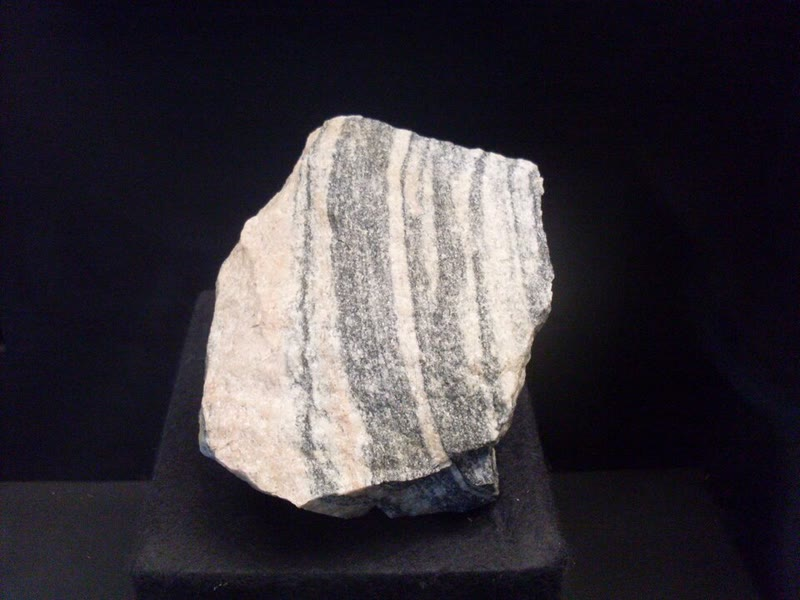
\includegraphics[height=4.6cm]{images/book2/g12-pedro-acasta-gneiss.jpg}\hspace{0.04\linewidth}%
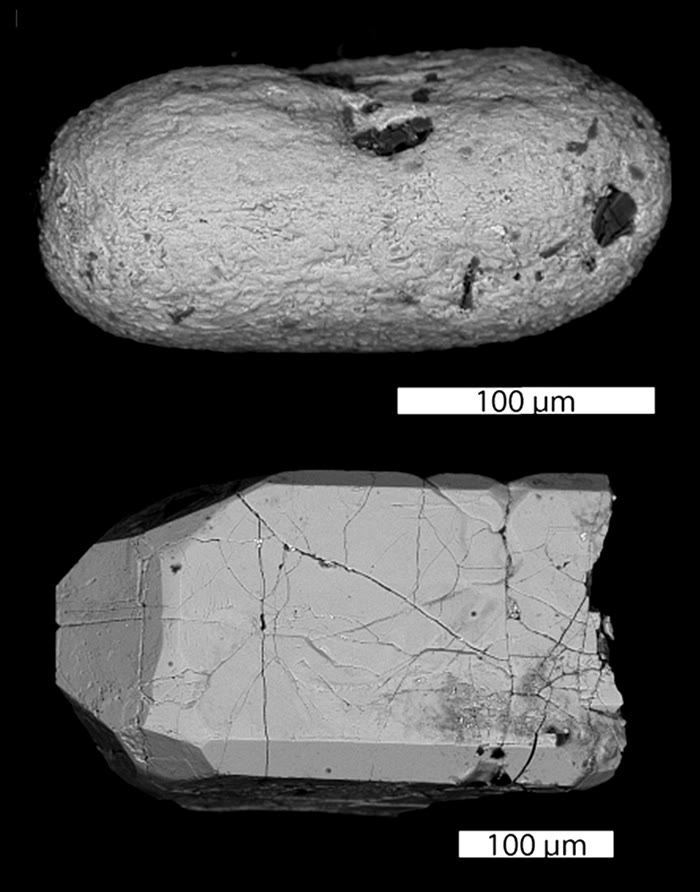
\includegraphics[height=4.6cm]{images/book2/g12-cavosie-jack-hills-zircons.jpg}

{\small À esquerda: um pedaço do gnaisse de Acasta, com 4.03 bilhões de
anos, exposto num museu. Fotografia Pedroalexandrade (CC~BY-SA~3.0). À
direita: dois grãos de zircão das Jack Hills, na Austrália Ocidental, vistos
ao microscópio eletrônico; cada barra de escala mede \qty{100}{\micro m}. O
grão de cima foi arredondado ao ser transportado pela água, o de baixo
conservou as faces do cristal. Imagens A.~Cavosie e J.~Valley (domínio
público).}
\end{omfigure}
% ledger: photo:g12-acasta, photo:g12-jack-hills-zircons

\begin{recall}
A crosta termina no \omterm{def:g11:seismic-structure:moho}{Moho}, abaixo do qual fica o manto, mais denso
(\cref{ch:g11:seismic-structure}). A \omterm{def:g11:ocean-ridges:oceanic-lithosphere}{crosta oceânica} tem cerca de
\qty{7}{km} de basalto e de \omterm{def:g11:ocean-ridges:gabbro}{gabro} formados nas dorsais
(\cref{ch:g11:ocean-ridges}), e nunca tem mais de cerca de 190 milhões de
anos (\cref{ch:g11:drift-to-spreading}). As camadas externas flutuam sobre a
\omterm{def:g11:lithosphere-asthenosphere:lithosphere}{astenosfera}: no modelo de Airy, uma região que fica a uma altura $h$ acima
tem uma crosta mais espessa de $h\,\rho_m/(\rho_m -
\rho_c)$ (\cref{ch:g11:lithosphere-asthenosphere}). As rochas ígneas são
nomeadas pela sua \omterm{def:g11:igneous-rocks:texture}{textura} e pelo seu teor de sílica: \omterm{def:g11:igneous-rocks:felsic-mafic}{máficas} de 45 a
\qty{55}{\percent} de \ce{SiO2}, \omterm{def:g11:igneous-rocks:felsic-mafic}{intermediárias} de 55 a 65, \omterm{def:g11:igneous-rocks:felsic-mafic}{félsicas} de 65 a
75 (\cref{ch:g11:igneous-rocks}). Os elementos radioativos decaem a uma taxa
constante, o que dá às rochas as suas idades (os livros de física;
\cref{ch:g12:age-of-the-earth}).
\end{recall}
% ledger: white92:crust, data:b2-seafloor-age, tulane:magma-types

\section{Do que são feitos os continentes}

\begin{definition}[Crosta continental]\label{def:g12:continental-crust:continental-crust}
A \emph{crosta continental}\index{crosta continental} é a crosta que forma
os continentes, incluindo as suas partes que ficam sob mares rasos. Ela é
espessa, de composição granítica em média na sua parte superior, leve, e
pode ser muito antiga.
\end{definition}
% ledger: tulane:crust-types, tulane:roots, cogley84:continents

Os continentes são maiores que as terras emersas. As bordas da \omterm{def:g12:continental-crust:continental-crust}{crosta
continental} ficam sob o mar, nas plataformas continentais: mapeada assim, a
\omterm{def:g12:continental-crust:continental-crust}{crosta continental} cobre \num{210}~milhões~de~\unit{km^2}, \qty{41}{\percent}
da superfície da Terra, dos quais quase um terço, \qty{30.6}{\percent}, está
submerso. Contando as suas partes submersas, a altitude média da \omterm{def:g12:continental-crust:continental-crust}{crosta
continental} fica só cerca de \qty{120}{m} acima do nível do mar.
% ledger: cogley84:continents

Na superfície, os continentes mostram todo tipo de rocha --- sedimentos,
\omterm{def:g11:igneous-rocks:volcanic-plutonic}{rochas vulcânicas}, rochas metamórficas ---, mas, sob a cobertura
sedimentar, a \omterm{def:g12:continental-crust:continental-crust}{crosta continental} é feita principalmente de rochas graníticas
e das rochas metamórficas e \omterm{def:g11:igneous-rocks:volcanic-plutonic}{plutônicas} de antigas \omterm{def:g12:continental-crust:root}{raízes} de montanhas. Em
média, a \omterm{def:g12:continental-crust:continental-crust}{crosta continental} inteira contém \qty{60.6}{\percent} de sílica; a
sua parte superior é mais rica, \qty{66.6}{\percent}, logo a sua parte mais
profunda deve ser mais pobre.
% ledger: rg14:crust, tulane:crust-types, cm95:crust

\begin{omfigure}
\begin{tikzpicture}
\begin{axis}[omrecord, ybar=0pt, width=0.92\linewidth, height=5.0cm, bar width=7pt,
  ymin=0, ymax=80, ylabel={fração da massa (\unit{\percent})},
  symbolic x coords={SiO2, Al2O3, FeO, MgO, CaO, Na2O, K2O},
  xticklabels={\ce{SiO2}, \ce{Al2O3}, \ce{FeO}, \ce{MgO}, \ce{CaO}, \ce{Na2O}, \ce{K2O}},
  xtick=data, enlarge x limits=0.08, ymajorgrids=true, xmajorgrids=false,
  legend style={font=\scriptsize, at={(0.98,0.97)}, anchor=north east, legend columns=1}]
% ledger: rg14:crust (upper and bulk continental crust; FeO* total iron)
\addplot[fill=omLithGranite, draw=black!60] coordinates {(SiO2,66.6) (Al2O3,15.4) (FeO,5.04) (MgO,2.48) (CaO,3.59) (Na2O,3.27) (K2O,2.80)};
\addplot[fill=omProp!55, draw=black!60] coordinates {(SiO2,60.6) (Al2O3,15.9) (FeO,6.71) (MgO,4.66) (CaO,6.41) (Na2O,3.07) (K2O,1.81)};
% ledger: earle:magma-oxides (mafic magma: midpoint of each range, the bar spans the range)
\addplot[fill=omLithBasalt, draw=black!60, error bars/.cd, y dir=both, y explicit]
  coordinates {(SiO2,50) +- (0,5) (Al2O3,16) +- (0,2) (FeO,10) +- (0,2) (MgO,7) +- (0,2) (CaO,9) +- (0,2) (Na2O,2) +- (0,1) (K2O,1.75) +- (0,1.25)};
\legend{crosta continental superior, crosta continental inteira, magma máfico (faixa)}
\end{axis}
\end{tikzpicture}

{\small Composição da \omterm{def:g12:continental-crust:continental-crust}{crosta continental} comparada com a de um magma \omterm{def:g11:igneous-rocks:felsic-mafic}{máfico},
o tipo que forma a \omterm{def:g11:ocean-ridges:oceanic-lithosphere}{crosta oceânica}: os principais óxidos, em porcentagem da
massa (\ce{FeO} conta todo o ferro). A \omterm{def:g12:continental-crust:continental-crust}{crosta continental} é mais rica em
sílica, sódio e potássio, mais pobre em ferro, magnésio e cálcio. Dados:
Rudnick e Gao (2014); faixa \omterm{def:g11:igneous-rocks:felsic-mafic}{máfica} segundo S.~Earle, \emph{Physical
Geology} (CC~BY~4.0).}
\end{omfigure}
% ledger: rg14:crust, earle:magma-oxides

\section{Uma crosta espessa e leve}

Os levantamentos sísmicos encontram o \omterm{def:g11:seismic-structure:moho}{Moho} sob os continentes a
profundidades muito diferentes. Em média sobre todos os continentes,
ponderada pela área, a crosta tem cerca de \qty{41}{km} de espessura; ela é
mais fina, cerca de \qty{30}{km}, onde foi estirada, e mais espessa, cerca
de \qty{46}{km} em média, nos cinturões de montanhas. Longe dos cinturões de
montanhas, ela tem comumente de 35 a \qty{40}{km}; sob as cadeias mais
altas, de 50 a \qty{70}{km}, cerca de \qty{70}{km} sob partes do Tibete. A
\omterm{def:g11:ocean-ridges:oceanic-lithosphere}{crosta oceânica} tem cerca de \qty{7}{km} de espessura: a \omterm{def:g12:continental-crust:continental-crust}{crosta continental}
é de cinco a dez vezes mais espessa.
% ledger: cm95:crust, tulane:roots, karplus:tibet-moho, white92:crust

\begin{omfigure}
\begin{tikzpicture}
\begin{axis}[omrecord, xbar, bar shift=0pt, width=0.78\linewidth, height=5.0cm, bar width=8pt,
  xmin=0, xmax=80, ymin=0.4, ymax=5.6, ytick={1,...,5},
  yticklabels={crosta oceânica, continentes estirados, continentes (média), cordilheiras (média), sob o Tibete},
  xlabel={espessura da crosta (\unit{km})}, ymajorgrids=false,
  nodes near coords, nodes near coords style={font=\scriptsize, anchor=west}, point meta=explicit symbolic]
% ledger: white92:crust, cm95:crust, karplus:tibet-moho
\addplot[fill=omLithBasalt, draw=black!60] coordinates {(7.1,1) [7.1]};
\addplot[fill=omLithGranite, draw=black!60] coordinates {(30.5,2) [30.5] (41.1,3) [41.1] (46.3,4) [46.3] (70,5) [uns 70]};
\end{axis}
\end{tikzpicture}

{\small Espessura da crosta segundo medições sísmicas. Dados: White,
McKenzie e O'Nions (1992) para a \omterm{def:g11:ocean-ridges:oceanic-lithosphere}{crosta oceânica}; Christensen e Mooney
(1995) para as médias continentais; Karplus e colaboradores (2019) para o
Tibete.}
\end{omfigure}
% ledger: white92:crust, cm95:crust, karplus:tibet-moho

A \omterm{def:g12:continental-crust:continental-crust}{crosta continental} é também leve. A sua densidade média é de cerca de
\qty{2830}{kg/m^3}. O basalto e o \omterm{def:g11:ocean-ridges:gabbro}{gabro} da \omterm{def:g11:ocean-ridges:oceanic-lithosphere}{crosta oceânica}, ricos em
piroxênio e em olivina, chegam a cerca de \qty{3000}{kg/m^3}
(\cref{ch:g11:minerals}), e o manto logo abaixo do \omterm{def:g11:seismic-structure:moho}{Moho} a cerca de
\qty{3380}{kg/m^3}. Uma crosta espessa e leve flutua alto: é por isso que
os continentes ficam acima do fundo oceânico, e que um continente não pode
ser arrastado para baixo numa \omterm{def:g11:subduction-zones:subduction}{zona de subducção}. Onde um continente chega a
uma fossa, ele é leve demais para afundar; a \omterm{def:g11:subduction-zones:subduction}{subducção} para, e os dois
continentes colidem (\cref{ch:g12:mountain-building}). A \omterm{def:g12:continental-crust:continental-crust}{crosta
continental}, uma vez formada, é difícil de destruir.
% ledger: cm95:crust, data:prem, tulane:roots, tulane:no-subduct
% values (mineral_density.py): basalt/gabbro rock line 3.0015 g/cm3

\begin{omfigure}
\begin{tikzpicture}[x=1cm, y=0.075cm, font=\footnotesize]
  % continental column: 41 km of crust, surface at +0.12 km (mean height); ocean column: 3.7 km of water drawn schematically
  \fill[omLithGranite] (0,0) rectangle (3,-41);
  \fill[omLithPeridotite!60] (0,-41) rectangle (3,-60);
  \fill[omSea] (6,0) rectangle (9,-4);
  \fill[omLithGabbro] (6,-4) rectangle (9,-11.1);
  \fill[omLithPeridotite!60] (6,-11.1) rectangle (9,-60);
  \draw[black!60] (0,0) rectangle (3,-60) (6,0) rectangle (9,-60);
  \draw[line width=0.9pt] (0,-41) -- (3,-41) (6,-11.1) -- (9,-11.1);
  \node[align=center] at (1.5,-20) {crosta continental\\cerca de \qty{41}{km}\\\qty{2830}{kg/m^3}\\até 4 bilhões de anos};
  \node[align=center] at (7.5,-24) {manto\\\qty{3380}{kg/m^3}\\abaixo do Moho};
  \node[align=center] at (1.5,-50.5) {manto};
  \node at (7.5,-2) {oceano};
  \draw[black!60] (8.6,-7.6) -- (9.3,-7.6);
  \node[anchor=west, align=left] at (9.3,-7.6) {crosta oceânica, cerca de \qty{7}{km}\\\qty{3000}{kg/m^3}\\menos de 200 milhões de anos};
  \node[anchor=east] at (-0.1,-41) {Moho};
  \node[anchor=east] at (5.9,-11.1) {Moho};
  \node[anchor=south] at (1.5,0) {um continente};
  \node[anchor=south] at (7.5,0) {um oceano};
  \foreach \d in {0,20,40,60} {\draw[black!60] (-1.5,-\d) -- (-1.3,-\d); \node[anchor=east, font=\scriptsize] at (-1.5,-\d) {\d};}
  \draw[black!60] (-1.4,0) -- (-1.4,-60);
  \node[rotate=90, font=\scriptsize] at (-2.3,-30) {profundidade (\unit{km})};
\end{tikzpicture}

{\small Um continente e um oceano lado a lado (profundidades em escala,
larguras não; o oceano desenhado com \qty{4}{km} de profundidade): a \omterm{def:g12:continental-crust:continental-crust}{crosta
continental} é mais espessa, mais leve e muito mais antiga que a \omterm{def:g11:ocean-ridges:oceanic-lithosphere}{crosta
oceânica}.}
\end{omfigure}
% ledger: cm95:crust, white92:crust, data:prem, bowring99:acasta, data:b2-seafloor-age

\begin{method}[Comparar a crosta continental e a crosta oceânica]\label{met:g12:continental-crust:compare}
Para saber que tipo de crosta fica sob um lugar, compare cinco propriedades:
\begin{enumerate}
  \item a espessura: cerca de \qty{7}{km} para a \omterm{def:g11:ocean-ridges:oceanic-lithosphere}{crosta oceânica}, de 30 a
        \qty{70}{km} para a \omterm{def:g12:continental-crust:continental-crust}{crosta continental};
  \item as rochas: basalto e \omterm{def:g11:ocean-ridges:gabbro}{gabro}, ou granito, gnaisse e rochas aparentadas,
        sob uma cobertura de sedimentos;
  \item a composição: cerca de \qty{50}{\percent} de sílica, ou cerca de 60
        e mais;
  \item a densidade: cerca de \qty{3000}{kg/m^3}, ou cerca de \qty{2830}{kg/m^3};
  \item a idade: menos de 200 milhões de anos, ou até 4 bilhões de anos.
\end{enumerate}
A altitude é um indício, não um teste: a maior parte do fundo oceânico fica
a quilômetros de profundidade, mas as bordas dos continentes ficam sob mares
rasos.
\end{method}
% ledger: white92:crust, cm95:crust, rg14:crust, earle:magma-oxides, cogley84:continents

\begin{example}[Um fundo de mar raso]\label{ex:g12:continental-crust:shelf}
Um navio de pesquisa encontra um fundo de mar a \qty{150}{m} de
profundidade. Perfis sísmicos põem o \omterm{def:g11:seismic-structure:moho}{Moho} a \qty{32}{km} abaixo do fundo do
mar; um testemunho de sondagem traz, sob os sedimentos, uma rocha de grãos
grossos feita de quartzo, feldspato e mica. Que crosta fica ali?

\emph{Solução.} Espessura de cerca de \qty{32}{km}: continental, mais fina
que a média, como onde foi estirada. Um granito sob os sedimentos:
continental. O fundo do mar é uma plataforma continental, uma das partes
submersas que formam quase um terço dos continentes.
\end{example}
% invented numbers; ledger: cm95:crust, cogley84:continents

Quanto pesa toda essa crosta? Uma camada fina em comparação com o raio da
Terra tem uma massa simples.

\begin{proposition}[A massa de uma camada fina]\label{prop:g12:continental-crust:thin-layer}
Uma camada de espessura $H$ e de densidade $\rho$ que cobre uma fração $f$
da superfície de um planeta de raio $R \gg H$ e de densidade média
$\bar\rho$ tem uma massa $m \approx 4\pi R^2 f H \rho$, e a sua parte na
massa $M$ do planeta é
\[
  \frac{m}{M} \approx 3 f\,\frac{H}{R}\,\frac{\rho}{\bar\rho}.
\]
\end{proposition}
% ledger: earth:Rmean, earth:density

\begin{proof}
A superfície do planeta é $4\pi R^2$; a camada cobre $4\pi R^2 f$ e, sendo
fina, tem um volume próximo dessa área vezes $H$, logo $m \approx 4\pi R^2
f H \rho$. A massa do planeta é $M = \tfrac{4}{3}\pi R^3 \bar\rho$. Dividindo,
$m/M \approx 4\pi R^2 f H \rho / (\tfrac{4}{3}\pi R^3 \bar\rho) = 3 f (H/R)
(\rho/\bar\rho)$.
\end{proof}

Para a \omterm{def:g11:ocean-ridges:oceanic-lithosphere}{crosta oceânica} --- os \qty{59}{\percent} restantes da superfície,
\qty{7.1}{km}, cerca de \qty{3000}{kg/m^3} ---, com $R = \qty{6371}{km}$ e
$\bar\rho = \qty{5513}{kg/m^3}$, a parte é $3 \times 0.59 \times
(7.1/6371) \times (3000/5513) \approx 0.0011$: cerca de um décimo de por
cento da massa da Terra. O problema de fim de semana faz o mesmo para os
continentes.
% ledger: cogley84:continents, white92:crust, earth:Rmean, earth:density

\section{Uma crosta antiga}

O fundo oceânico é jovem em toda parte: três quartos dele têm menos de 100
milhões de anos, e quase nada tem mais de 190 milhões de anos. Com os
continentes é outra história. As suas rochas cobrem quase toda a história
da Terra, do gnaisse de Acasta, com 4.03 bilhões de anos, às lavas que
entram em erupção hoje, e grãos de zircão levam o registro até 4.4 bilhões
de anos.
% ledger: data:b2-seafloor-age, bowring99:acasta, uw14:jack-hills

\begin{omfigure}
\begin{tikzpicture}
\begin{axis}[omrecord, ybar interval, width=0.82\linewidth, height=5.0cm,
  xmin=0, xmax=200, ymin=0, ymax=0.12, xtick={0,20,...,200},
  xlabel={idade do fundo oceânico (milhões de anos)},
  ylabel={parte do fundo oceânico}, yticklabel style={/pgf/number format/fixed},
  ymajorgrids=true, xmajorgrids=false, clip=false, x tick label as interval=false]
% computed in figdata/grade-12/crust_ages.py (Seton 2020 grid, 1-degree cells, area-weighted)
\addplot[fill=omDef!35, draw=omDef] table[x=age_lo, y=share] {figdata/out/grade-12-crust_ages-hist.dat};
\node[anchor=north east, align=right, font=\scriptsize, fill=white, inner sep=2pt] at (axis cs:198,0.115)
  {rocha continental mais antiga: \num{4030} milhões de anos,\\vinte vezes mais antiga que o fundo oceânico mais antigo};
\end{axis}
\end{tikzpicture}

{\small Que idade tem o fundo oceânico: a parte da sua área em cada faixa
de 10 milhões de anos. O fundo jovem domina; quase nada tem mais de 190
milhões de anos (algumas bacias antigas do leste do Mediterrâneo foram
deixadas de fora). Dados: Seton e colaboradores (2020), calculados.}
\end{omfigure}
% ledger: data:b2-seafloor-age, bowring99:acasta
% values (crust_ages.py): oldest_open_myr 192.5, share_younger_100 0.765, share_younger_150 0.956, rock_over_floor 20.9

As partes mais antigas dos continentes formam os seus núcleos.

\begin{definition}[Cráton]\label{def:g12:continental-crust:craton}
Um \emph{cráton}\index{craton@cráton} é um núcleo antigo e estável de um
continente: \omterm{def:g12:continental-crust:continental-crust}{crosta continental} formada e deformada há mais de um bilhão de
anos, que desde então esfriou e não se deforma mais. As suas rochas são
principalmente rochas metamórficas e \omterm{def:g11:igneous-rocks:volcanic-plutonic}{plutônicas}, as \omterm{def:g12:continental-crust:root}{raízes} profundas de
antigas montanhas.
\end{definition}
% ledger: tulane:cratons

Em volta dos \omterm{def:g12:continental-crust:craton}{crátons} ficam cinturões de rochas deformadas mais jovens, as
\omterm{def:g12:continental-crust:root}{raízes} erodidas de cadeias de montanhas construídas mais tarde; os
cinturões tendem a ser mais jovens em direção às bordas de um continente.
Um continente cresceu por formação de montanhas que soldou crosta nova às
suas bordas, em volta de um núcleo antigo. No Canadá, onde as rochas do
\omterm{def:g12:continental-crust:craton}{cráton} ficam na superfície, afloram gnaisses e granitos de 1 a 3 bilhões de
anos, aqui à beira de um lago.
% ledger: tulane:cratons, photo:g12-canadian-shield

\begin{omfigure}
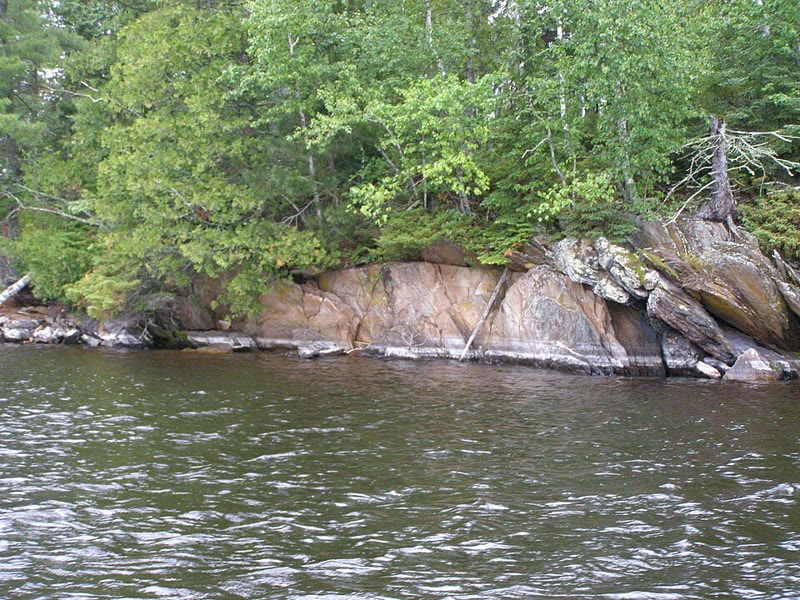
\includegraphics[height=5.0cm]{images/book2/g12-light-canadian-shield.jpg}

{\small Gnaisses e granitos de 1 a 3 bilhões de anos à beira de um lago no
Canadá, parte do núcleo antigo da América do Norte. Fotografia Chris Light
(CC~BY-SA~4.0).}
\end{omfigure}
% ledger: photo:g12-canadian-shield

Por que a \omterm{def:g12:continental-crust:continental-crust}{crosta continental} dura, enquanto o fundo oceânico é sempre
jovem? A \omterm{def:g11:ocean-ridges:oceanic-lithosphere}{crosta oceânica} é densa: ela volta a afundar no manto nas \omterm{def:g11:subduction-zones:subduction}{zonas de
subducção}, e nada dela sobrevive muito além de 200 milhões de anos. A
\omterm{def:g12:continental-crust:continental-crust}{crosta continental} é leve demais para afundar; ela pode ser desgastada pela
erosão, estirada ou amarrotada, mas fica na superfície. As rochas de um
continente são um arquivo de quatro bilhões de anos.
% ledger: tulane:no-subduct, tulane:roots, data:b2-seafloor-age

\section{As raízes das montanhas}

Quanto mais altas as montanhas, mais espessa a crosta sob elas.

\begin{definition}[Raiz de uma cadeia de montanhas]\label{def:g12:continental-crust:root}
A \emph{raiz}\index{raiz (de uma cadeia de montanhas)} de uma cadeia de
montanhas é a parte da sua crosta espessada que desce no manto abaixo do
nível do \omterm{def:g11:seismic-structure:moho}{Moho} sob as planícies em volta.
\end{definition}
% ledger: tulane:roots

O modelo de Airy prevê a \omterm{def:g12:continental-crust:root}{raiz}: uma cadeia que fica a $h$ acima do seu
entorno tem uma \omterm{def:g12:continental-crust:root}{raiz} $r = h\,\rho_c/(\rho_m - \rho_c)$, cerca de cinco vezes
a sua altura com $\rho_c = \qty{2830}{kg/m^3}$ e $\rho_m =
\qty{3380}{kg/m^3}$ (\cref{prop:g11:lithosphere-asthenosphere:airy}). Dois
tipos de medição veem as \omterm{def:g12:continental-crust:root}{raízes}. Os levantamentos sísmicos encontram o \omterm{def:g11:seismic-structure:moho}{Moho}
mais fundo sob as cadeias: de 50 a \qty{70}{km} sob muitos cinturões de
montanhas, cerca de \qty{70}{km} sob partes do Tibete. A gravidade é mais
fraca sobre as cadeias de montanhas do que sugeriria a sua massa visível: a
\omterm{def:g12:continental-crust:root}{raiz} leve, no lugar de um manto mais denso, cria um déficit de massa em
profundidade, e as anomalias de gravidade medidas acompanham a topografia e
a espessura da crosta encontrada pela sismologia. Os continentes flutuam, e
as suas montanhas flutuam mais alto.
% ledger: tulane:roots, karplus:tibet-moho, cm95:crust, data:prem

\section{Exercícios}

\begin{exercise}[$\star$]\label{exo:g12:continental-crust:1}
Copie e complete para a \omterm{def:g12:continental-crust:continental-crust}{crosta continental} e para a \omterm{def:g11:ocean-ridges:oceanic-lithosphere}{crosta oceânica}:
espessura; principais rochas; teor de sílica; densidade; idade máxima.
\end{exercise}

\begin{exercise}[$\star$]\label{exo:g12:continental-crust:2}
A \omterm{def:g12:continental-crust:continental-crust}{crosta continental} inteira contém \qty{60.6}{\percent} de sílica, a sua
parte superior \qty{66.6}{\percent}. Usando as classes de sílica das rochas
ígneas, cada uma é \omterm{def:g11:igneous-rocks:felsic-mafic}{máfica}, \omterm{def:g11:igneous-rocks:felsic-mafic}{intermediária} ou \omterm{def:g11:igneous-rocks:felsic-mafic}{félsica}? Cite uma \omterm{def:g11:igneous-rocks:volcanic-plutonic}{rocha
plutônica} de mesma composição.
\end{exercise}

\begin{exercise}[$\star$]\label{exo:g12:continental-crust:3}
Por que a \omterm{def:g11:ocean-ridges:oceanic-lithosphere}{crosta oceânica} pode afundar no manto numa \omterm{def:g11:subduction-zones:subduction}{zona de subducção}, e a
\omterm{def:g12:continental-crust:continental-crust}{crosta continental} não? Responda com densidades.
\end{exercise}

\begin{exercise}[$\star$]\label{exo:g12:continental-crust:4}
(1) O que é um \omterm{def:g12:continental-crust:craton}{cráton}? (2) Que idade têm, no mínimo, as rochas de um \omterm{def:g12:continental-crust:craton}{cráton}?
(3) Que tipos de rocha o formam?
\end{exercise}

\begin{exercise}[$\star$]\label{exo:g12:continental-crust:5}
O fundo oceânico mais antigo tem cerca de 190 milhões de anos, o gnaisse de
Acasta 4.03 bilhões de anos. Quantas vezes o gnaisse é mais antigo? Por que
não existe fundo oceânico tão antigo?
\end{exercise}

\begin{exercise}[$\star\star$]\label{exo:g12:continental-crust:6}
A \omterm{def:g12:continental-crust:continental-crust}{crosta continental} cobre \num{210.4}~milhões~de~\unit{km^2}, dos quais
\qty{30.6}{\percent} ficam sob o mar. (1) Que área de \omterm{def:g12:continental-crust:continental-crust}{crosta continental}
fica sob o mar? (2) Que área fica acima dele? (3) A superfície da Terra é
$4\pi R^2$ com $R = \qty{6371}{km}$. Que parte da superfície a \omterm{def:g12:continental-crust:continental-crust}{crosta
continental} cobre?
\end{exercise}

\begin{exercise}[$\star\star$]\label{exo:g12:continental-crust:7}
Calcule a massa de uma coluna de crosta de \qty{1}{m^2} de seção, da
superfície até o \omterm{def:g11:seismic-structure:moho}{Moho}: (1) através de \qty{41.1}{km} de \omterm{def:g12:continental-crust:continental-crust}{crosta continental}
a \qty{2830}{kg/m^3}; (2) através de \qty{7.1}{km} de \omterm{def:g11:ocean-ridges:oceanic-lithosphere}{crosta oceânica} a
\qty{3000}{kg/m^3}. (3) Quantas vezes a primeira é mais pesada?
\end{exercise}

\begin{exercise}[$\star\star$]\label{exo:g12:continental-crust:8}
Uma cadeia fica a \qty{2.5}{km} acima de planícies cuja crosta tem
\qty{35}{km} de espessura. Com $\rho_c = \qty{2830}{kg/m^3}$ e $\rho_m =
\qty{3380}{kg/m^3}$, calcule a sua \omterm{def:g12:continental-crust:root}{raiz} e a espessura da sua crosta. O
resultado está na faixa medida sob os cinturões de montanhas?
\end{exercise}

\begin{exercise}[$\star\star$]\label{exo:g12:continental-crust:9}
A partir do histograma das idades do fundo oceânico: (1) que parte do fundo
oceânico tem menos de 30 milhões de anos? (2) Que faixa de 10 milhões de
anos contém mais fundo? (3) Por que a parte cai em direção às idades
antigas?
\end{exercise}

\begin{exercise}[$\star\star$]\label{exo:g12:continental-crust:10}
Mapeada com as suas partes submersas, a \omterm{def:g12:continental-crust:continental-crust}{crosta continental} tem uma altitude
média de cerca de \qty{120}{m}. Suponha que as suas partes submersas,
\qty{30.6}{\percent} da sua área, ficam em média a \qty{100}{m} abaixo do
nível do mar. Qual é a altitude média da sua parte emersa? Por que as
estimativas mais antigas, que contavam só as terras emersas, dão uma
altitude média muito maior?
\end{exercise}

\begin{exercise}[$\star\star$]\label{exo:g12:continental-crust:11}
Um furo de sondagem numa ilha longe no meio de um oceano atinge, abaixo de
algumas centenas de metros de lavas, um \omterm{def:g11:ocean-ridges:gabbro}{gabro}; perfis sísmicos põem o \omterm{def:g11:seismic-structure:moho}{Moho} a
\qty{8}{km} de profundidade. Outro furo de sondagem, sob uma planície larga e
plana, atinge gnaisse a \qty{2}{km}, e o \omterm{def:g11:seismic-structure:moho}{Moho} fica a \qty{38}{km} de
profundidade. Use o método para decidir que crosta fica sob cada um.
\end{exercise}

\begin{exercise}[$\star\star\star$]\label{exo:g12:continental-crust:12}
Quão boa é a aproximação da proposição? (1) Calcule o volume exato de uma
casca de espessura \qty{41.1}{km} na superfície de uma esfera de raio
\qty{6371}{km}, $\tfrac{4}{3}\pi\bigl(R^3 - (R - H)^3\bigr)$, e o volume
aproximado, $4\pi R^2 H$. (2) Qual é a diferença relativa? Compare-a com
$H/R$.
\end{exercise}

\begin{exercise}[$\star\star\star$]\label{exo:g12:continental-crust:13}
Suponha que o terço superior da \omterm{def:g12:continental-crust:continental-crust}{crosta continental}, em massa, contém
\qty{66.6}{\percent} de sílica, e a crosta inteira \qty{60.6}{\percent}. (1)
Qual é o teor de sílica dos dois terços inferiores? (2) A que classe de
rocha ígnea ele corresponde? (3) O que isso diz sobre a \omterm{def:g12:continental-crust:continental-crust}{crosta continental}
profunda?
\end{exercise}

\begin{exercise}[$\star\star\star$]\label{exo:g12:continental-crust:14}
Suponha que nova \omterm{def:g11:ocean-ridges:oceanic-lithosphere}{crosta oceânica} se forma nas dorsais a cerca de
\qty{3}{km^2} por ano, e que o fundo oceânico cobre cerca de
\num{300}~milhões~de~\unit{km^2}. (1) Quanto tempo as dorsais levariam para
produzir uma área igual à de todo o fundo oceânico? (2) Compare com as
idades do fundo oceânico. (3) O que deve acontecer com o fundo antigo?
\end{exercise}

\begin{exercise}[$\star\star\star$]\label{exo:g12:continental-crust:15}
Suponha que toda a \omterm{def:g12:continental-crust:continental-crust}{crosta continental}, \qty{8.6e9}{km^3}, se formou a uma
taxa constante desde 4.0 bilhões de anos atrás. (1) Calcule a taxa em
quilômetros cúbicos por ano. (2) Os zircões das Jack Hills mostram que já
existia alguma crosta há 4.4 bilhões de anos. Uma taxa constante combina
com um mundo em que a maior parte da crosta poderia ter se formado cedo, ou
tarde? O que as rochas mais antigas poderiam contar, e o que não podem,
dado que a crosta antiga pode ser erodida ou reciclada?
\end{exercise}

\section{Problema: quanto pesa a crosta continental?}

\begin{problem}[{Problema de fim de semana --- a massa dos continentes}]
\label{pb:g12:continental-crust:1}
% ledger: cogley84:continents, cm95:crust, earth:mass, earth:Rmean, earth:density, white92:crust
% values: 4 pi R^2 = 5.1006e8 km2; V = 210.4e6 x 41.1 = 8.647e9 km3; m = 2.447e22 kg; m/M = 0.410 %
A \omterm{def:g12:continental-crust:continental-crust}{crosta continental} cobre \num{210.4}~milhões~de~\unit{km^2} (partes
submersas incluídas). Os levantamentos sísmicos lhe dão uma espessura média
de \qty{41.1}{km} e uma densidade média de \qty{2830}{kg/m^3}. A Terra tem
um raio médio de \qty{6371}{km}, uma massa de \qty{5.9722e24}{kg} e uma
densidade média de \qty{5513}{kg/m^3}.

\medskip
\noindent\textbf{Parte I --- A área.}
\begin{enumerate}
  \item Calcule a área da superfície da Terra, $4\pi R^2$, em
        \unit{km^2}.
  \item Que parte dela a \omterm{def:g12:continental-crust:continental-crust}{crosta continental} cobre?
  \item \qty{30.6}{\percent} da \omterm{def:g12:continental-crust:continental-crust}{crosta continental} ficam sob o mar. Que área
        é essa?
  \item Que área da superfície da Terra sobra para a \omterm{def:g11:ocean-ridges:oceanic-lithosphere}{crosta oceânica},
        supondo que o resto é todo oceânico?
  \item Por que a \omterm{def:g12:continental-crust:continental-crust}{crosta continental} é maior que as terras emersas?
\end{enumerate}

\medskip
\noindent\textbf{Parte II --- Espessura e volume.}
\begin{enumerate}[resume]
  \item Por que o volume pode ser calculado como área vezes espessura,
        embora a crosta fique sobre uma esfera?
  \item Calcule o volume da \omterm{def:g12:continental-crust:continental-crust}{crosta continental} em \unit{km^3}.
  \item Converta-o em \unit{m^3}.
  \item Outra estimativa da espessura média é \qty{36}{km}. Que volume ela
        dá?
  \item Em quanto por cento os dois volumes diferem?
\end{enumerate}

\medskip
\noindent\textbf{Parte III --- Densidade e massa.}
\begin{enumerate}[resume]
  \item Calcule a massa da \omterm{def:g12:continental-crust:continental-crust}{crosta continental} com \qty{41.1}{km}.
  \item Calcule a massa de uma coluna de \qty{1}{m^2} através da \omterm{def:g12:continental-crust:continental-crust}{crosta
        continental}.
  \item Calcule a massa da \omterm{def:g11:ocean-ridges:oceanic-lithosphere}{crosta oceânica}: área da questão~4, espessura
        \qty{7.1}{km}, densidade \qty{3000}{kg/m^3}.
  \item Qual é mais pesada, e quantas vezes? Por que, embora cubra uma área
        menor?
  \item Por que a \omterm{def:g12:continental-crust:continental-crust}{crosta continental} é menos densa que a \omterm{def:g11:ocean-ridges:oceanic-lithosphere}{crosta oceânica}?
\end{enumerate}

\medskip
\noindent\textbf{Parte IV --- Em comparação com a Terra.}
\begin{enumerate}[resume]
  \item Divida a massa da questão~11 pela massa da Terra.
  \item Verifique o resultado com a proposição sobre as camadas finas.
  \item Que parte da massa da Terra é a \omterm{def:g11:ocean-ridges:oceanic-lithosphere}{crosta oceânica}?
  \item A \omterm{def:g12:continental-crust:continental-crust}{crosta continental} contém as únicas rochas com mais de cerca de
        200 milhões de anos. Que parte da massa da Terra carrega o registro
        de quase toda a sua história?
  \item Conclua: que parte da massa da Terra é a \omterm{def:g12:continental-crust:continental-crust}{crosta continental}?
\end{enumerate}
\end{problem}
